\documentclass[10pt,a4paper]{article}

\usepackage[utf8x]{inputenc}
\usepackage[english]{babel}
\usepackage[T1]{fontenc,url}
\usepackage[hang,small,bf]{caption}
\usepackage{relsize}
\usepackage{setspace}
\usepackage{parskip}
\usepackage{lmodern}
\usepackage{microtype}
\usepackage{verbatim}
\usepackage{amsmath, amssymb, amsthm}
\usepackage{mathtools}
\usepackage{tikz}
\usepackage{physics}
\usepackage{algorithm}
\usepackage{algpseudocode}
\usepackage{listings}
\usepackage{enumerate}
\usepackage{graphicx}
\usepackage{float}
\usepackage{hyperref}
\usepackage{varioref}
\usepackage{siunitx}
\usepackage{todonotes}
\usepackage{color}
\usepackage[margin=3cm]{geometry}
\labelformat{equation}{equation~(#1)}

\renewcommand{\exp}{\mathrm{e}^}
\newcommand{\halflife}{t_{\frac{1}{2}}}
\newcommand{\half}{\frac{1}{2}}
\newcommand{\planck}{$h = \SI{6.626e-34}{J.s}$}

\definecolor{light_green}{rgb}{0, 0.6, 0}
\definecolor{light_grey}{rgb}{0.5, 0.5, 0.5}
\definecolor{magenta}{rgb}{0.7, 0, 0.5}


\lstdefinestyle{py}{
    language = python,
    frame = single,
    showstringspaces = false,
    basicstyle = \small\ttfamily,
    breaklines = true,
    commentstyle = \color{light_grey},
    keywordstyle = \color{magenta},
    stringstyle = \color{light_green},
}

\begin{document}

\section*{Exercise 9.1 - Acceleration class}
\addcontentsline{toc}{section}{Exercise 9.1 - Acceleration class - \texttt{Jerk.py}}

The file \texttt{constant\_acceleration\_class.py} contains a class \texttt{ConstantAcceleration} for calculating one dimensional movement with constant acceleration, using the equations of movement. The constructor saves the initial position, velocity, and acceleration. The class call returnes the position at a given time \texttt{t}, and the method \texttt{velocity} returns the velocity at a given time \texttt{t}.

The purpose of this exercise is to expand the functionality of the \texttt{ConstantAcceleration} class into a \texttt{LinearAcceleration} class, which can also deal with cases were the acceleration is a first order polynomial on the form $a = a_0 + jt$. The constant $j$ is known as "jerk", and is the change in acceleration over time. The equations of movement now look like
\[	x(t) = x_0 + v_0t + \half a_0t^2 + \frac{1}{6}jt^3
\]
\[	v(t) = v_0 + a_0t + \half jt^2
\]

Make a class \texttt{LinearAcceleration}, which borrows the functionality of \texttt{ConstantAcceleration}, but with the added ability to calculate with a given jerk. Wether you implement a 'has-a' or 'is a' relationship between the two classes are up to you, but you must borrow code from the \texttt{ConstantAcceleration} class as much as possible.

Filename: \texttt{Jerk.py}



\section*{Exercise 9.2 - Solids}
\addcontentsline{toc}{section}{Exercise 9.2 - Solids - \texttt{Solid.py}}
% Kanskje utvide med Young, eventuelt lage egen for kap. 7. vet ikke helt ennå
In this exercise we will look at how we can made a simple model of an arbitrary solid and then a specific type of solid using inheritance. 

\subsection*{a)}
Define a class \texttt{Solid} which takes the volume of a body as parameter to the constructor.
Let the class have a function which calculates the density of the body where the mass of the body is given as parameter to the function. Recall that the density is defined to be mass divided by volume. 

\subsection*{b)}
Define a class \texttt{Iron} which is a subclass of \texttt{Solid}. 
The constructor must take the volume of a given body (made of iron) and mass as parameters. \\
Define a function in \texttt{Iron} which calls the function from \texttt{Solid} to calculate and returns the density of the created body. 

\subsection*{c)}
Define a test function which initialize an instance of the class from b) with volume \SI{0.1}{\cubic\meter} and mass 787 kg and test if the calculated density is \SI{7870}{\kg.\per\cubic\meter}. Remember to call your testfunction!

Filename: \texttt{Solid.py}
 
\section*{Exercise 9.3 - Moment of inertia about center of mass}
\addcontentsline{toc}{section}{Exercise 9.3 - Moment of inertia about center of mass - \texttt{Moment\_of\_inertia.py}}
The mass of a body can be looked upon as being a measurement of how difficult it is to change its velocity. We have a similar measure for rotation of a body, namely the \textit{moment of inertia} about the center of mass of the body\footnote{The center of mass of a body is a position in space dependent on the distribution of mass within the shape of the body.}. 
\subsection*{a)}
Define a class which represents a geometric object. The constructor must only take the mass $M$ of the object as parameter. 

Initialize an instance of this class with $M = 5\,$kg.
\subsection*{b)}
Write a class which inherits from the class defined in a). This class will represent a cylindrical object. The constructor must take as parameters the mass $M$ of the object and its radius $R$.


Define a function inside this class which calculates and returns the moment of inertia to the cylindrical object. The moment of inertia $I$ to a cylinder with mass $M$ and radius $R$ is found (by calculation) to be:
\[
I = \frac{1}{2}MR^2
\] 

Initialize an instance of this class with $M = \SI{5}{\kg}$ and $R = \SI{0.75}{\meter}$ and display its moment of inertia. 
\subsection*{c)}
Make a class which inherits from the class in b). This class shall represents a cylindrical shell with mass $M$ and radius $R$. 
\begin{center}
	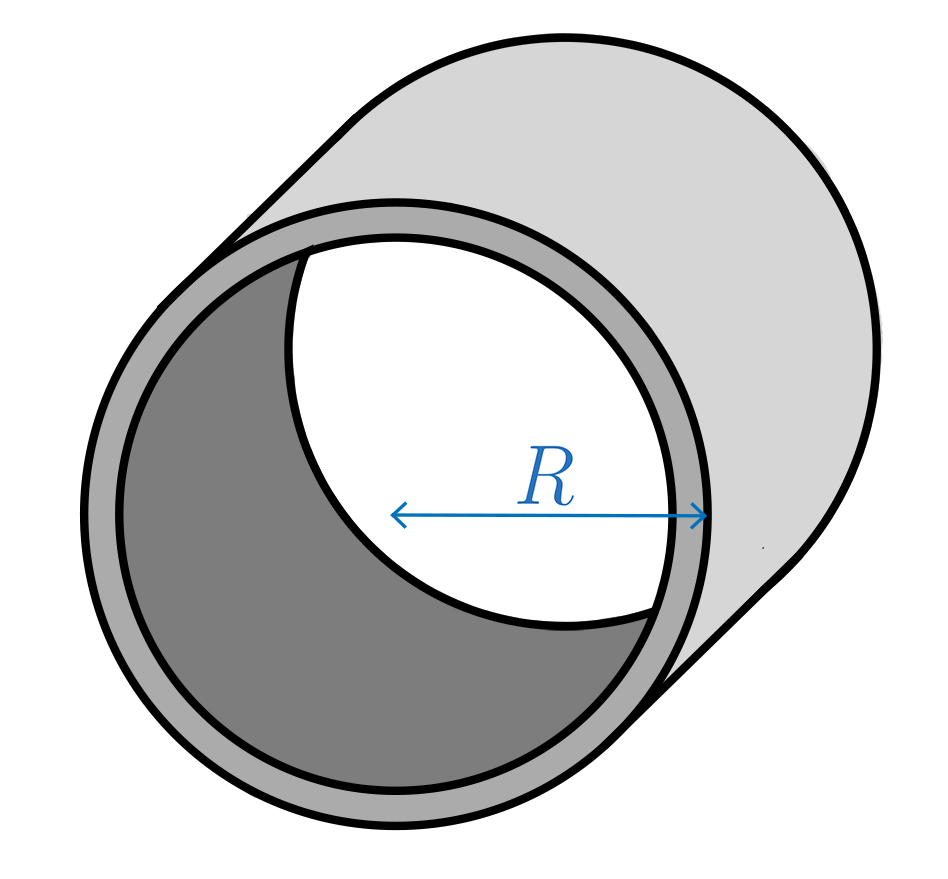
\includegraphics[scale=.5]{fig_sylinderskall-cp1.png}
	\captionof{figure}{Illustration of a cylindrical shell with radius $R$.}
\end{center}

This class must also be able to calculate and return the value of the moment of inertia of the cylindrical shell. However, in this case we can the moment of inertia calculated in the class from b). You see, it can be shown that the moment of inertia for a cylindrical shell is:
\[
I = MR^2
\]
We could therefore make b) calculate the moment of inertia, and then multiply its answer by 2. 

Initialize an instance of this class representing a cylindrical shell with $M = \SI{5}{\kg}$ and $R = \SI{0.75}{\meter}$ and write out its moment of inertia. 

\textbf{Remark:} In this subtask you are supposed to write very little code. Exploit inheritance as much as possible!

Filename: \texttt{Moment\_of\_inertia.py}


\end{document}
